\section{Implementation Details}
\label{app:implementation_details}

\subsection{Robot Platforms} 
We evaluate \textsc{LAP-3B} across four robot embodiments that differ in kinematics, sensing configurations, and control interfaces:
\begin{itemize}
\item \textbf{DROID}: a seen embodiment during pre-training, comprising a 7-DoF arm with both external and wrist-mounted cameras.
\item \textbf{Custom Franka}: an unseen 7-DoF arm with external and wrist-mounted cameras, featuring a novel gripper and wrist camera mounting that differ from Franka robots observed during training.
\item \textbf{YAM}: an unseen 6-DoF arm with a single external camera.
\item \textbf{Kinova}: an unseen 7-DoF arm with external and wrist-mounted cameras.
\end{itemize}

For fine-tuning, we use joint-space actions on YAM to enable more precise low-level control, while all other robots are controlled using end-effector pose actions.




\subsection{Training Hyperparameters} 
\begin{wraptable}{r}{0.4\textwidth}
    \centering
    \small
    % \vspace{-10pt}
    \vspace{-1.2cm}
    \caption{Training Hyperparameters for LAP-3B.}
    \label{tab:hyperparams}
    \renewcommand{\arraystretch}{1.15}
    \begin{tabular}{l c}
    \toprule
    \textbf{Hyperparameter} & \textbf{Value} \\
    \midrule
    Batch size & 2048 \\
    Learning rate & $1 \times 10^{-4}$ \\
    Warmup steps & 5000 \\
    EMA start step & 5000 \\
    EMA decay & 0.999 \\
    Action horizon & 16 \\
    Adam $(\beta_1, \beta_2)$ & $(0.9,\ 0.95)$ \\
    Gradient clipping norm & 1.0 \\
    Weight decay & $1 \times 10^{-4}$ \\
    \bottomrule
    \end{tabular}
    \vspace{-8pt}
\end{wraptable}
The overall training objective is:
\[
\mathcal{L} = \mathcal{L}_{\text{flow}} + \lambda \mathcal{L}_{\text{CE}}.
\]

We use $\lambda=0.8$ during pre-training and $\lambda=0.4$ during fine-tuning. Other hyper-parameters is shown in Table.\ref{tab:hyperparams}. We set $\lambda<1$ during pre-training to slightly downweight the language-action loss, as it converges substantially faster than the diffusion-based action expert. This balancing prevents the faster language-action objective from dominating optimization and encourages both components to learn at comparable rates.


\subsection{Baseline Implementations}
For all replicated baselines ($\pi_{0.5}$-replicated, $\pi_{0}$-replicated, and VLA-0-replicated), we carefully tune hyperparameters and select the best-performing checkpoints based on preliminary real-robot validation runs. 
Across all baselines, we sweep the learning rate over $\{1\times10^{-4}, 5\times10^{-5}\}$ and the batch size over $\{1024, 2048\}$. 
For $\pi_{0.5}$-replicated, we additionally sweep the cross entropy loss weight of the FAST tokens over $\{0.1, 0.4, 0.6, 0.8\}$ and the action horizon over $\{16, 32\}$.

% \begin{wraptable}{r}{0.4\textwidth}
%     \centering
%     \small
%     \vspace{-10pt}
%     \caption{Training Hyperparameters for LAP-3B.}
%     \label{tab:hyperparams}
%     \renewcommand{\arraystretch}{1.15}
%     \begin{tabular}{l c}
%     \toprule
%     \textbf{Hyperparameter} & \textbf{Value} \\
%     \midrule
%     Batch size & 2048 \\
%     Learning rate & $1 \times 10^{-4}$ \\
%     Warmup steps & 5000 \\
%     EMA start step & 5000 \\
%     EMA decay & 0.999 \\
%     Action horizon & 16 \\
%     Adam $(\beta_1, \beta_2)$ & $(0.9,\ 0.95)$ \\
%     Gradient clipping norm & 1.0 \\
%     Weight decay & $1 \times 10^{-4}$ \\
%     \bottomrule
%     \end{tabular}
%     \vspace{-8pt}
% \end{wraptable}

Unless otherwise specified, the final hyperparameters used for all replicated baselines are a batch size of $2048$, learning rate of $1\times10^{-4}$, action horizon of $16$, and loss weight of $\lambda=0.6$.

Beyond these explicitly tuned parameters, all replicated baselines share the same design choices as our method, including identical network architectures, data mixtures, sampling strategies, and optimization settings. 
All remaining hyper-parameters follow those listed in Table~\ref{tab:hyperparams}.

For $\pi_{0}$-replicated, we directly follow the original OpenPI codebase implementation \cite{black2024pi0visionlanguageactionflowmodel}. 

For $\pi_{0.5}$-replicated, we extend the original implementation to include supervision of the VLM backbone using FAST action tokens and Knowledge Insulation \cite{driess2025knowledgeinsulatingvisionlanguageactionmodels} (stop gradient from the action expert to the backbone), which is not provided in the released code. 

For VLA-0-replicated, we reimplement the method strictly following the specifications in the original paper~\cite{goyal2025vla0buildingstateoftheartvlas}, including masked action augmentation, the recommended action resolution, and prompt format. We additionally perform careful hyperparameter tuning beyond what is reported in the paper, particularly for learning rate and batch size. With these adjustments, the replicated model achieves comparable performance on the LIBERO benchmark; however, it does not scale to large-scale datasets, as discussed in Section.\ref{subsec:zero_shot}.

\subsection{Prompt and Language-Action Format}
For both our model and all baselines, the prompt follow a structured template:

\begin{tcolorbox}[promptbox]
Task: \texttt{<instruction>}, predict the robot's action in the \texttt{<base frame>} or \texttt{<end-effector frame>}; State: \texttt{$s_1$\ $s_2$\ \ldots\ $s_D$}; Answer:
\end{tcolorbox}

An example example is:

\begin{tcolorbox}[promptbox]
Task: Put the marker into the cup, predict the robot's action in the base frame; State: 20 121 34 144 112 45 235 44 21 255; Answer:
\end{tcolorbox}

Language-actions are generated as structured clauses in fixed order:

\begin{tcolorbox}[promptbox]
\texttt{move <direction> <k> cm; tilt <direction> <k> degrees; rotate <cw/ccw> <k> degrees; open/close gripper}
\end{tcolorbox}

Translational magnitudes are discretized into integer centimeters and rotational magnitudes in integer degrees, with zero-valued movements omitted to suppress near-zero control noise.

\subsection{Motion Prediction VQA Data Generation}
Analogous to language–action data curation, motion prediction VQA pairs are generated automatically without manual annotation. Each training instance is constructed using the following prompt template:
\begin{tcolorbox}[promptbox]
Task: \texttt{question}; State: \texttt{$s_1$\ $s_2$\ \ldots\ $s_D$}; Answer:
\end{tcolorbox}
\noindent where the \texttt{question} ask the model to describe the temporal relationship between two observations (e.g., \emph{“What movement did the robot make from the first image to the second in the robot base frame?”}). We randomly sample semantically equivalent question phrasings to increase prompt diversity and robustness. The corresponding answer is given by the ground-truth language–action describing the robot motion between the two frames.

\subsection{Image Pre-processing and Augmentation}
All input images are first resized (with padding) to a fixed resolution before further processing. During training, we apply augmentation to images from all camera views. Images are normalized to $[0,1]$ and transformed using a composed pipeline consisting of a random crop to $95\%$ of the target resolution followed by resizing back to the original size, a random in-plane rotation sampled uniformly from $[-5^\circ, 5^\circ]$, and color jitter with brightness, contrast, and saturation parameters each set to $0.2$ (corresponding to multiplicative factors sampled uniformly from $[0.8, 1.2]$). The augmented images are then rescaled back to $[-1,1]$ for model input. Each image in the batch is augmented using an independent random seed. For VQA samples, augmentation is skipped entirely to preserve the original visual input.


\subsection{Attention Mask} 
\begin{wrapfigure}{r}{0.44\linewidth}
    \centering
    % \vspace{-12pt}
    \vspace{-1.7cm}
    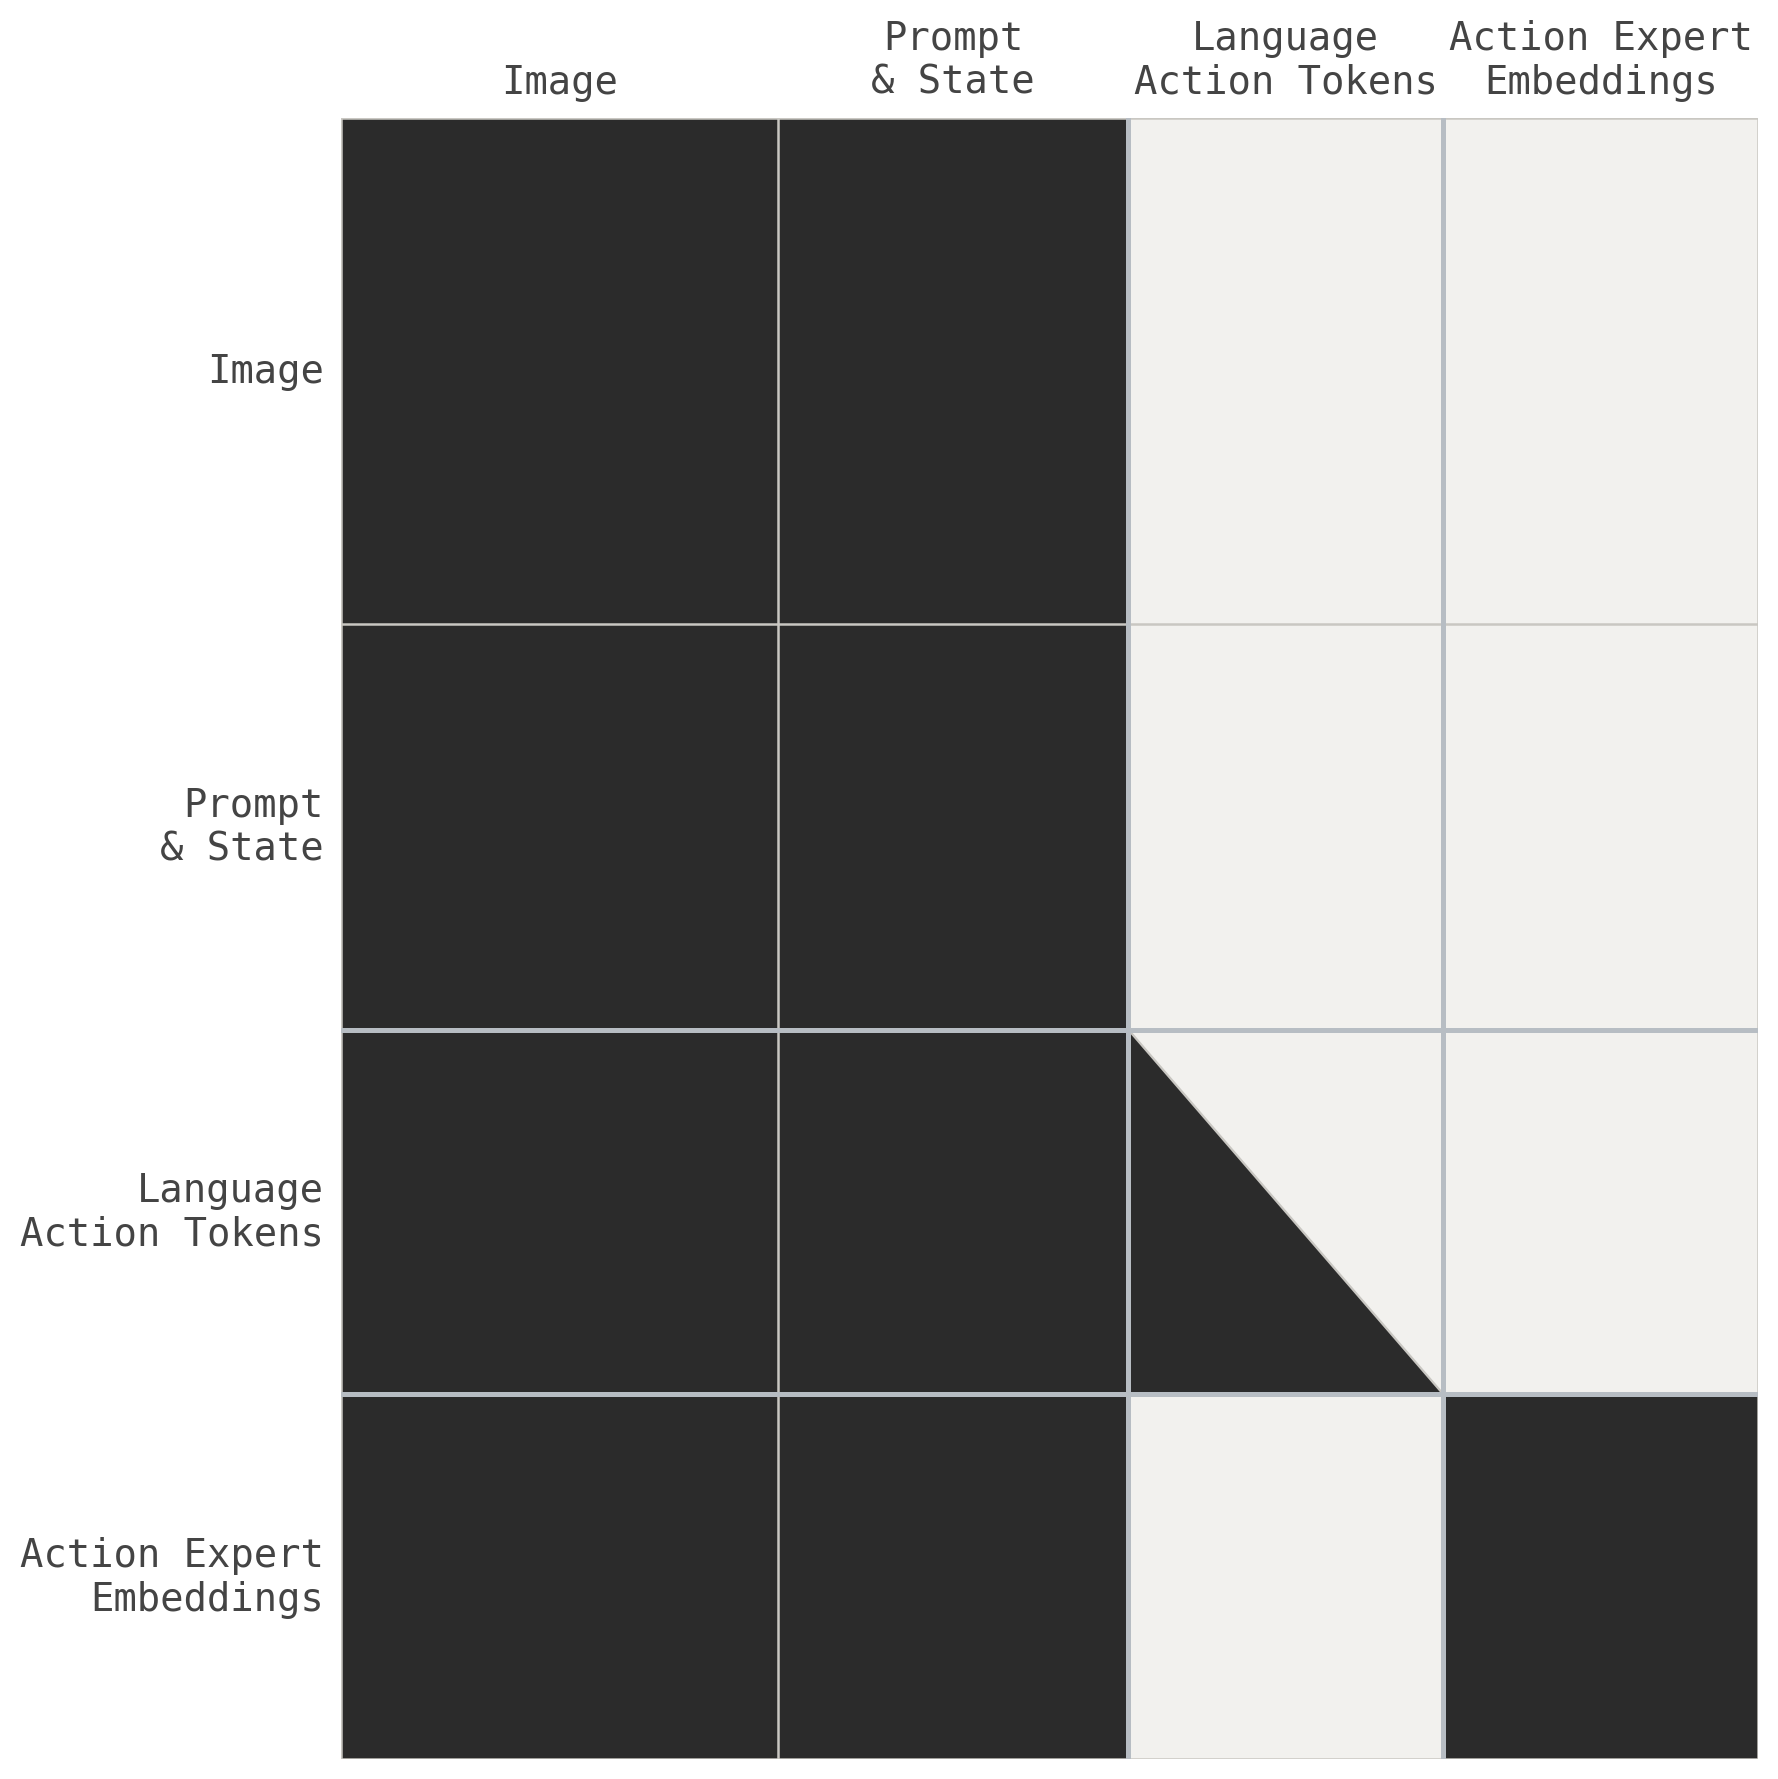
\includegraphics[width=\linewidth]{figures/appendix/fig10_attention_mask.png}
    \captionsetup{skip=3pt}
    \caption{Attention mask visualization for LAP-3B.}
    \label{fig:attention-mask}
    \vspace{-6pt}
\end{wrapfigure}
We visualize the attention mask of \textsc{LAP-3B} in Fig.~\ref{fig:attention-mask}. Prefix tokens—including image, prompt, and state—use bidirectional attention. Language-action tokens attend causally to one another while having full attention to all prefix tokens. The action expert uses full self-attention and fully attends to prefix tokens, but does not attend to language-action tokens.

